\svnid{$Id: grundlagen.tex 108 2012-05-12 18:44:01Z dgens001 $}
\chapter{Projektgrundlagen}

\textit{Dieses Kapitel bietet eine kurze Übersicht über definierte Ziele und Rahmenbedingungen. Es bietet
einen ersten Architekturüberblick und stellt grobe Systembestandteile mit ihren Zuständigkeiten dar.}

\section{Zielsetzung}
Ziel des Projekts ist eine selbst entwickelte Spieleapplikation, die ohne
aufwändige Grafikdarstellung oder KI einen amüsanten Zeitvertreib bieten
kann. Nicht ganz nebenbei soll die Applikation Ergebnis eines größeren
Projekts sein, an dem sich softwaretechnische Methoden, kollaborative Arbeit
und der nahezu vollständige Entwicklungszyklus üben und testen lassen.
Fachliche, technische und andere qualitative Ziele sollen in diesem Dokument
zusammengefasst werden.

\section{Inhaltlicher Überblick}
Die Autoren dieser Spezifikation haben sich darauf verständigt, ein Spiel nach der Machart einiger
bereits bekannter Roleplaying-Adventure zu entwickeln. Das Spiel könnte also (je nach Storyline) endlos 
spielbar sein, oder ein festes Ende haben, wobei das hier spezifierte Spiel einen definiertes Spielende
haben wird.
Um einen gewissen Anreiz für den \gls{Spieler} zu schaffen, sollte die Storyline 
diesen relativ frei durch den \gls{Campus} führen. Dabei wird es in späteren Erweiterungen
möglich sein, den eigenen \gls{Charakter} zu leveln. Inhaltliches Ziel soll das Finden
eines bestimmten \gls{Schein}s sein.
Der Spieler befindet sich immer auf genau einem \gls{Feld}. Er kann nur mit \glspl{Item} oder \gls{npcs}, die
sich auf dem gleichen \gls{Feld} befinden interagieren. Zudem hat er die Möglichkeit zu einem direkt 
benachbarten \gls{Feld} zu wechseln. Mehrere Felder bilden einen \gls{Raum}. \glspl{Raum} sind in sich 
geschlossene Areale. Räume haben einen oder mehrere \glspl{Eingang} und müssen dem \gls{Spieler} nicht 
zugänglich sein. Alle Räume zusammen bilden den \gls{Campus}. 
Von Zeit zu Zeit sollte der \gls{Spieler} einen oder mehrere Gegenstände (sog. \glspl{Item}) erhalten, die er
in seinen \gls{Inventar} aufnehmen kann. Manche \glspl{Item} sind wertvoll (hilfreich für den Verlauf des 
Spiels), andere nicht. Einige \glspl{Item} sollten sich kombinieren lassen, oder in anderer Form mit 
dem \gls{Spieler} oder der \gls{Welt} interagieren können. Der \gls{Spieler} sollte ein \gls{Savegame} 
anlegen und laden können. Das \gls{Savegame} beinhaltet die Campuskonfiguration und alle Elemente, die sich im
Spiel befinden. Es hat ein Datum und eine Versionsnummer (für den Fall einer Erweiterung).

\section{Technische Anforderungen}
Die Applikation soll unter Java Swing entwickelt werden. Sie sollte auf 
aktuellen Desktop-PCs ohne Leistungsprobleme spielbar sein (10MB freier 
Festplattenspeicher, 1GB RAM, 2GHz DualCore, 128MB Grafikspeicher, 
Bildschirmauflösung 1280x1024). Die Applikation sollte im Fenstermodus mit einer Fenstergröße von 1024x768
laufen und nicht vergrößer- oder verkleinerbar sein (entspricht Seitenverhältnis 4:3).
Der Fokus soll aber nicht auf möglichst realistischer Echtzeitgrafik, sondern auf dem Spielerlebnis liegen.
Darüber hinaus sollte der Spielplan anhand einer Spielplandatei konfigurierbar sein. 
Dort sollte man zunächst Wände und Spielstart, später vielleicht auch \acrlong{npc} und \glspl{Item} 
positionieren können.

\section{Architektur}
Die Anwendungslogik soll derart beschaffen sein, dass der Spieler anhand einfacher Zugriffe (3-4 Klicks)
zu den gesuchten Funktionen findet. Ziel ist nicht, dem Spieler über möglichst viele Einstellungsmöglichkeiten
verfügen zu lassen. Es gibt ein Itemsystem, ein Raumsystem und ein Dialogsystem. In eventuellen Erweiterungen
können zusätzliche Systeme implementiert werden. Die Architektur sollte später in Darstellung, Logik und 
Anwendungsdaten systematisch unterteilt werden. Generell lässt sich das Spiel inhaltlich in zwei Modi 
unterteilen, Ingame- und \gls{Menuemodus}. Der Menümodus sollte der Standardmodus sein, in dem die Applikation
startet und von dem aus man in den Ingamemodus gelangt. Der Einfachheit halber sind die Abbruchsübergänge in
Abbildung \ref{fig:zustaende_entwurf} nicht berücksichtigt.

\begin{figure}[h]
	\begin{center} 
		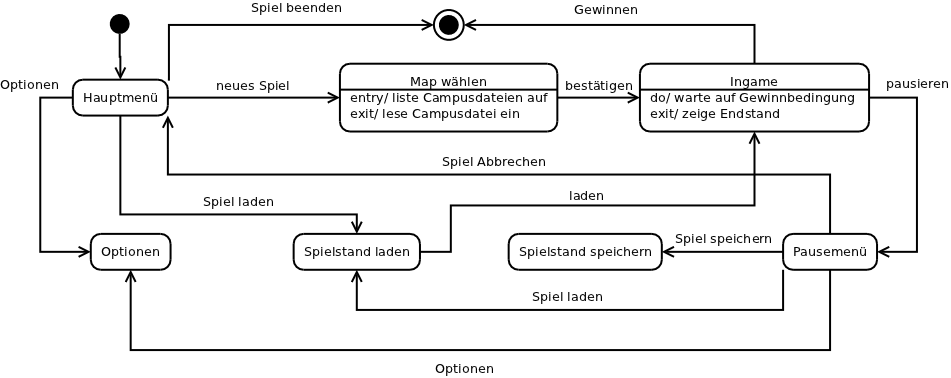
\includegraphics[width=150mm, height=60mm]
                  {kapitel/grundlagen/architektur.png}
	\end{center}
	\caption{grobe Struktur der Systemzustände}
	\label{fig:zustaende_entwurf}
\end{figure}

\section{Erweiterbarkeit}
Der \gls{Charakter} kann in späteren Erweiterungen z.B. verschiedene Fähigkeiten oder
Eigenschaften haben. Diese könnten dann im Laufe des Spiels weiterentwickelt werden 
(z.B. anhand sog. CreditPoints). CreditPoints würde man durch das erfolgreiche Sammeln
der \glspl{Schein} erhalten, mehrere \glspl{Schein} könnten dann ein Semester ergeben.
Es könnte dann auch einen Abschluss in Form eines höchsten Semesters (z.B. Master of Sciene) geben.
Wahlweise könnte der \gls{Spieler} dann trotz Erreichen dieses Semesters weiterhin 
durch die \gls{Welt} navigieren und zufällig auftauchende \glspl{Schein} (z.B. durch Lösen von
Minispielen oder Rätseln) finden. Es könnte dann auch die Möglichkeit geben, unabhängig von den 
\glspl{Savegame} Charakterprofile zu speichern, zu editieren und zu laden. Daher soll es möglich sein, 
die Gegenstände, Objekte und Charaktere im Spiel von Version zu Version zu ergänzen und zu erweitern. 
So könnten in einer zukünftigen Erweiterung der NPCs feste Routen vorgesehen werden, auf denen diese sich
wärend dem Spiel bewegen.
